% This is a template following IEEE style
\documentclass[conference]{IEEEtran}

\usepackage{cite}
\usepackage{amsmath,amssymb,amsfonts}
\usepackage{algorithmic}
\usepackage{graphicx}
\usepackage{textcomp}
% code listings package
\usepackage{listings}
% these packages render tables
\usepackage{booktabs}
% the package for references
% \usepackage[hidelinks]{hyperref}
\usepackage{listings}

% force columns to be level on last page (for easier printing in journals)
\usepackage{flushend}
% code highlighting. found in the pandoc default

% override tightlist. error with pandoc?
\def\tightlist{}

% start the document, the markdown code takes over from this point
\begin{document}
\title{Recursive Parallel Methods for Fast 2D Matrix Initialization and Transposition}

\newcommand{\AuthorName}{Christian Kauten}
\newcommand{\AuthorEmail}{jck0022@auburn.edu}

\newcommand{\Deptartment}{Software Engineering and Computer Science}
\newcommand{\University}{Auburn 
University}
\newcommand{\Location}{Auburn, AL, USA}

\author{
  \IEEEauthorblockN{\AuthorName}
  \IEEEauthorblockA{\textit{\Deptartment} \\
  \textit{\University}\\
  \Location \\
  \AuthorEmail}
}

\maketitle

\begin{abstract}

Modern computers use clever tricks to increase performance without incurring
massive financial costs. One such performance improvement is seen in
hierarchical memory where a series of progressively slower memory devices work
together to reduce the latency induced by memory operations. Although these
systems work well when used effectively, naive code can break the system,
resulting in bad performance. These issues become highly apparent when looping
over large matrices. Depending on the architecture of the cache, the ordering
of the matrix in memory, and the code itself, initializing and performing
actions on matrices could take a large amount of time. This paper explores the
effects of cache on matrix operations using C-code. The results show that
programmers need pay close attention to the design of their code to ensure
proper utilization of the underlying hardware through novel means.

\end{abstract}

\begin{IEEEkeywords}
Cache, Memory, Matrix, Transpose
\end{IEEEkeywords}

\section{Introduction}\label{introduction}

\subsection{Hierarchical Memory}\label{hierarchical-memory}

\emph{Hierarchical (Cache) memory} utilizes a sequence of memory devices
and heuristics to improve performance of memory operations. This
sequence exists to balance performance and cost, allowing machines to
take advantage of more expensive, but faster, memory devices. The
machine can then leverage these devices for recurring or frequently used
data to reduce latency.

\subsubsection{Locality}\label{locality}

In order to best utilize this hierarchy of devices, engineers employ two
similar, but distinct heuristics based on \emph{locality}.
\emph{Temporal locality} states that data used recently is likely to be
used again soon. Without temporal locality, cache hits would rarely
occur as new data from memory would always be needed. \emph{Spatial
locality} is the principle that data near recently used data is likely
to be needed soon. This principle drives engineers to copy surrounding
data to cache when a cache miss occurs for a memory address.

\section{Methodology}\label{methodology}

\subsection{Matrices}\label{matrices}

Matrices in C are stored in memory in row-major order. As such, they
flatten out in memory as a sequential vector of rows. The most efficient
way of \emph{iteratively} traversing this matrix is sequentially
iterating over each cell in each row in the vector. This is know as
\emph{row-wise} traversal. By properly utilizing spatial locality, it
performs better than \emph{column-wise} traversal. With large matrices,
column-wise traversal will generate more cache misses as the algorithm
wont portray the same degree of spatial locality. This is because each
cell in a different row is a full matrix length of data types away from
that cell in memory.

\subsection{Recursive Initialization}\label{recursive-initialization}

In order to speed up initialization, the base matrices are encoded as
piecewise functions based on the recursive series in the lower
triangular matrix in each. This allows the matrices to initialize out of
order as the incremental operator is no longer necessary. This encoding
allows for a recursive divide-and-conquer initialization function. This
function cuts the matrix into smaller sub-matrices and initializes them
one at a time. Using a base case of an appropriately small matrix, the
algorithm becomes ``cache naive''. This means that it effectively uses
the cache line without hardware specific blocking. Such a solution is
more general than a blocking solution designed for a specific chipset.

\subsubsection{Parallel Initializtion}\label{parallel-initializtion}

The recursive algorithm lends itself well to parallelism as there is no
need to lock for data access. The tux machines feature 8 physical cores
that allow 16 contiguous threads. Each core has its own L1 and L2 cache,
but share an L3 cache. As such, parallelism allows the software to
better utilize the entirety of the cache on the machine. Because the
machines are shared, the OS will have to schedule the processes across
multiple users. As such, the program may run better on sequential runs
as more resources are allocated by the OS for the single user account.

\subsection{Transpose}\label{transpose}

The transpose operator, \(M^T\), flips each value \(v_{i,j}\) in a 2D
matrix \(M\) by its \(i\) and \(j\) values. Many novel solutions exist
to speed up the transpose operation. The fastest solution has a time
complexity of \(O(1)\). Instead of directly computing the transpose, the
index can simply be inverted: \(i \leftarrow j, j \leftarrow i\). This
allows access to the transposed matrix with no change in memory. By
inverting the index, this solution also inverts the optimal way to
traverse the matrix from row-wise to column-wise. This makes optimizing
cache usage of matrix operations more difficult for the programmer as
the convention will switch from row-wise to column-wise in certain
states.

\subsection{Recursive Transpose}\label{recursive-transpose}

A recursive transpose operator divides a matrix into four even
submatrices and computes their transpose. The bottom-left and top-right
quadrants are then swapped. An alternative recursive solution performs
the standard tranpose, but in a divide-and-conquer fashion. This latter
solution allows effective cache line usage without additional swap
operations or complex indexing.

\subsubsection{Parallel Transpose}\label{parallel-transpose}

Much like the recursive intialization, the tranpose operation is also
easily paralellized. This again allows for \emph{more} cache and CPUs
operating on the memory.

\subsection{Results}\label{results}

With all improvements in place, the algorithm achieves a mean score of
\(\approx 6.4s\) using row-major ordering to initialize and transpose.
Fig. \ref{all-means} displays the mean time as it changes across the 5
trials of 7 experiments. The times drop slightly between sequential
executions of the program as the OS allocates more resources for the
user. Each trial demonstrates a gradual decrease in time with each
additional test. This attributes to cache hits as the same memory is
accessed by the same program during the same execution.

\begin{figure}[ht]
\centering
\label{all-means}
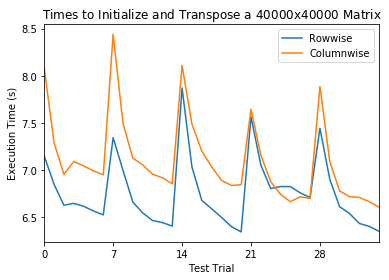
\includegraphics[height=2.5in]{img/all-means}
\end{figure}

\section{Conclusions}\label{conclusions}

This paper presents a recursive and parallel method to initialize and
transpose a 2x2 square matrix in minimal time. A key feature of this
recursive algorithm is a natural ``cache naive'' trait that allows it to
exploit the cache line without explicit cache blocking. This coupled
with a highly parallel architecture, like the 8-core Intel Core i7
processors in the Tux machines, allows the algorithm to initialize and
transpose a 40000x40000 matrix (\(\approx 12.8\)GB) in less than 7
seconds (\(\approx 1.8GB/s\)). Although this time is fast, faster times
certainly exist. Future research may investigate the integration of
vector architectures like GPUs to speedup the initialization and
transpose of matrices.
\end{document}
